The first question we want to tackle is: how worse is the sparsity in an EPHS compared to a LSHS?
We show that, in general, the sparsity of an EPHS is arbitrarily worse.
Intuitively, this occurs when shortest and efficient paths are unrelated. 
\anote{The current example uses the stronger notion of $r$-significant. I can create a very simple example with the weaker definition, but it looks like cheating.}

\begin{proposition}\label{prop:treelike}
For any $h$, we can construct a family of networks such that the sparsity of LSHS is $h$ and that of EPHS is arbitrarily worse than $h$.
\end{proposition}
\begin{proof}
First, we construct an example where the sparsity grows from $h$ to $h^2$.
Consider an $h$-ary tree rooted at $u$ with three levels, i.e., with $1+h+h^2$ nodes.
Now add a node $v$ with $h$ children as in Figure~\ref{fig:treelike}. 
The grandchildren of $v$ are the same as the grandchildren of $u$.

All the edges are bidirectional and have unit cost.
The lengths are as follows: $ux_i$ and $vy_i$ (dashed in Figure~\ref{fig:treelike}) are zero; $uv$ and from $y_i$ to the leafs is one; from $x_i$ to the leafs is three.
It is easy to see that the sparsity of a LSHS is $h+1$.

On the other hand, every leaf $w$ is a $2$-efficient path.
Indeed, it can be extended to $x_iw$ that is the shortest path from $x_i$ to $w$ with constraint 1.
All the leafs are in the ball $B_4(u)$, so the sparsity is at least $h^2$.

\begin{figure}
\caption{Example where the CHD is much larger than the HD}
\label{fig:treelike}
\centering
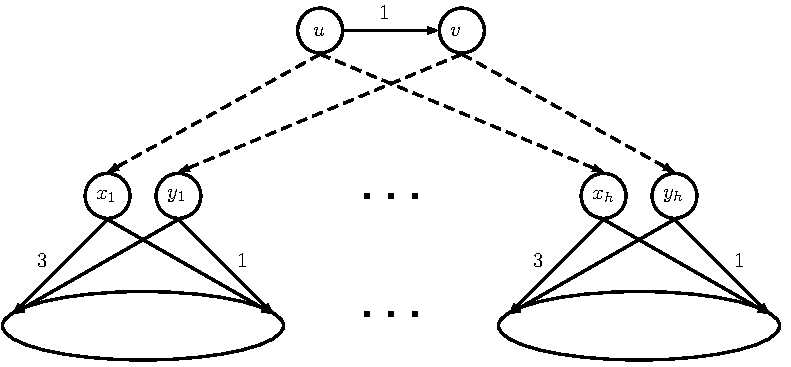
\includegraphics[scale=0.6]{TexImg/Treelike.pdf}
\end{figure}

The general case works in the same fashion.
We make the sparsity grow to $h^k$ by creating two complete, $k$-level, $h$-ary trees $T$ and $T'$.
Connect the root of $T$ to the root of $T'$ and the leafs of both trees are shared.
Observe that the number of nodes is 
\begin{align*}
n &=[\text{$k$-level $h$-ary tree}] + [\text{$(k-1)$-level $h$-ary tree}]\\
&= \frac{h^{k+1}-1}{h-1} + \frac{h^k-1}{h-1},
\end{align*}
therefore the sparsity is $\Theta(n)$, the worst possible.
\end{proof}

It is conjectured that road networks have small HD.
Is there evidence to conjecture small CHD in these networks?
We show how doubling dimension plus an additional property, defined bellow, do imply a positive answer.
A path $P'$ \emph{partially witnesses} $P$ if $P'\subseteq P$ and $P'$ is ``long enough''.
Formally, we define the following relation for path systems.

\begin{definition}
Let $\beta\geq 0$.
We say that a path system $\calQ'$ is a $\beta$-witness of the path system $\calQ$ if, for every $Q\in\calQ$, exists $Q'\in\calQ'$ such that $Q'\subseteq Q$ and $\ell(Q')\geq 2^{-\beta}\ell(Q)$.
\end{definition}

We explore first when the system of shortest paths $\calP$ is a partial witness for the system of efficient paths $\PE$.
At an intuitive level, the partial witness property says that efficient and shortest paths are not completely different, i.e., if $Q$ is efficient, some fraction of $Q$ is shortest.
As a consequence, an important node hitting numerous paths in $\calP$, should also hit many paths in $\PE$.
The bad examples in Proposition~\ref{prop:treelike} exploit networks that do not have partial witnesses.
We stress that doubling dimension depends only on $G$ and $\ell$; the partial witness property depends on the interplay between $G$, $c$ and $\ell$.
To get a bound using the partial witness, we relax the condition and ask only for long efficient paths to be witnessed.

\begin{proposition}\label{prop:doubling}
Assume $G$ is $\alpha$-doubling and $\calP$ is a $\beta$-witness for $\PE_r$ for every $r\geq \beta/2$.
If $(G,\ell)$ admits an $(h,r)$-LSHS for any $r$, then $(G,\ell,c)$ admits an $(\alpha^{\beta} h,r)$-EPHS for any $r$.
\end{proposition}
\begin{proof}
For any $r$, we need to construct a hitting set $C^E$ for $\calP_r^E$.
Assume first $r\geq\beta/2$.
Take $C$ as the hitting set for $\calP_{2^{-\beta}r}$, which is guaranteed to be sparse with respect to balls of radius $2^{-\beta+1}r$.
Define the desired set by
\[
C^E\defeq\{v\in C: v \text{ is in some $r$-efficient path} \}.
\]

Since $\calP$ is a $2^{-\beta}$-witness for $\PE$, $C^E$ is indeed a hitting set for $\PE_r$.
We are only left to prove the sparsity.
Take some $u\in V$, by doubling dimension we can cover $\Bf_{2r}(u)$ by at most $\alpha^\beta$ balls of radius $2^{-\beta+1}r$.
Each of these balls contains at most $h$ elements of $C$, therefore the sparsity is as claimed.
The argument for backward balls is identical.

Now we analyse the case $r<\beta/2$.
It is no longer true that the efficient paths are witnessed, but now the neigborhoods are small.
Since the edge lengths are integers, $\card{B_{2r}(v)}\leq \Delta^{2r}$.
Take $C=V$ \todo{finish this}
\end{proof}

\begin{remark}
The existence of a $\beta$-witness is not enough to bound the CHD.
Nevertheless, as discussed in Section~\ref{sec:multi_scale}, the existence of $(h,r)$-LSHS already allows the construction of HL.
\end{remark}
